\chapter{Metodologia}\label{metodologia}
% ---
Para a realização do embasamento deste trabalho, foram utilizadas tanto a metodologia de pesquisa bibliográfica 
quanto a de pesquisa documental. A primeira foi essencial para o levantamento de metodologias já consolidadas e 
amplamente estudadas, como as que serão abordadas no referencial teórico e, a seguir, nesta seção. Já a segunda 
foi empregada para identificar diferentes aplicações correlatas e para a elaboração do referencial teórico, além 
de ter sido utilizada na análise de dados internos do CECLIMAR, conforme comentado na conforme comentado na 
\hyperref[chapter:intro]{Introdução} deste trabalho.

Segundo \citeonline{gil2002elaborar}, a pesquisa bibliográfica é desenvolvida com base em materiais como livros 
e artigos científicos, ou seja, materiais já consolidados. Trata-se de uma pesquisa de grande importância, pois 
permite que os pesquisadores acessem diversos dados e informações dispersos que, individualmente, seriam muito 
trabalhosos e custosos de se coletar. Nesse tipo de pesquisa, entretanto, é necessário ter cuidado com citações 
de terceiros, que podem interpretar de forma equivocada algum dado ou informação originalmente levantados.

Ainda segundo o autor, a pesquisa documental se diferencia pela natureza das fontes de informação. Enquanto as 
pesquisas bibliográficas consistem essencialmente em um apanhado de contribuições de diversos autores sobre 
determinado assunto, a pesquisa documental ocorre por meio de materiais que ainda não receberam tratamento 
analítico ou que podem ser reelaborados, a depender dos objetos de pesquisa. As fontes da pesquisa documental 
são mais diversas e podem incluir conversas pessoais, entrevistas, documentos ou sites.

A metodologia de pesquisa bibliográfica foi realizada através da plataforma Google Scholar, publicações 
presentes no portal do Sistema de Informação sobre a Biodiversidade Brasileira (SiBBr), além de livros 
disponibilizados na biblioteca do Instituto Federal Campus Osório. Já a metodologia de pesquisa documental 
foi levantada a partir de arquivos internos, relatórios das Nações Unidas e conteúdos disponibilizados por 
desenvolvedores ou organizações que participaram do desenvolvimento das aplicações correlatas.

Após a fase de revisão bibliográfica se iniciará o desenvolvimento do sistema. Esta fase será realizada a 
partir do levantamento de requisitos junto de profissionais do CECLIMAR e, os requisitos levantados serão 
cadastrados e refinados para desenvolvimento cíclico do sistema. Cada ciclo visará a entrega de um produto 
com incrementos de requisitos pré estabelecidos. Ao final de cada um dos ciclos de desenvolvimento o sistema 
será disponibilizado para testes com servidores do CECLIMAR, os \textit{feedbacks} recebidos serão analisados, 
refinados e postos para desenvolvimento no ciclo seguinte. Um ponto de atenção no desenvolvimento desse 
sistema é que, por se tratar de um sistema de ciência cidadã, deve estar adequado com a LGPD para que possa 
ser publicado na Play Store para o uso da sociedade.

% ---
\section{Metodologia de desenvolvimento de \textit{software}}\label{sec:metodologia-desenv-software}
% ---

Para o desenvolvimento deste projeto foi escolhida uma abordagem de metodologia ágil relacionada 
ao ciclo iterativo incremental. Utilizando o \textit{Kanban} como método de gestão de fluxo de trabalho, a 
fim de melhorar a eficiência e qualidade do produto final a partir da visualização das tarefas. A 
ferramenta escolhida para realizar este gerenciamento foi o \textit{Jira}.

Segundo \citeonline{pressman2011engenharia}, os ciclos de desenvolvimento incremental podem ser 
divididos em 5 principais etapas: comunicação, planejamento, modelagem (análise e projeto), construção 
(codificação e testes) e emprego (entrega, \textit{feedback}). As etapas por ele descritas serão 
aplicadas neste projeto.

A comunicação será marcada por reuniões agendadas com os profissionais do CECLIMAR para definição de
 escopo e levantamento de requisitos do sistema. O planejamento será a análise, o refinamento e as 
 definições de quais funcionalidades serão desenvolvidas em cada ciclo. Durante a modelagem será 
 realizada a prototipação e análise dos pontos levantados na etapa anterior. Na construção será o 
 momento onde se dará a codificação e os testes da aplicação. E, por fim, durante o emprego o sistema 
 será disponibilizado para os profissionais do CECLIMAR e uma porcentagem de usuários que realizarão 
 testes e retornarão \textit{feedback} que serão analisados, catalogados e inseridos no \textit{Backlog} 
 para serem puxados em um ciclo posterior.

%  é necessária uma nota de rodape para explicar o que é o MVP??
O uso desta metodologia tem o objetivo de realizar uma primeira entrega que possa ser considerada um 
Mínimo Produto Viável (\textit{MVP}) atendendo aos requisitos básicos propostos inicialmente, mesmo que ainda 
se note a ausência de funcionalidades complementares. Esse \textit{MVP} se tornará então a base de avaliação que 
permitirá identificar necessidades adicionais e ajustes necessários. Com base nessa análise, é planejado 
o próximo incremento, ajustando a primeira entrega e adicionando novas funcionalidades conforme as necessidades.

Neste projeto foi montado um fluxo de trabalho no \textit{Jira} para desenvolvimento de \textit{software} visando 
auxiliar no processo e manter a visibilidade das tarefas de ponta a ponta. Para o \textit{workflow} principal, 
foi montado um esquema com \textit{Backlog}, Refinamento, Em desenvolvimento, Aguardando teste, Em teste, 
Correção de \textit{bugs} e \textit{Done} (Figura~\ref{fig:fluxoJira}).

\begin{figure}[htb]
    \centering
    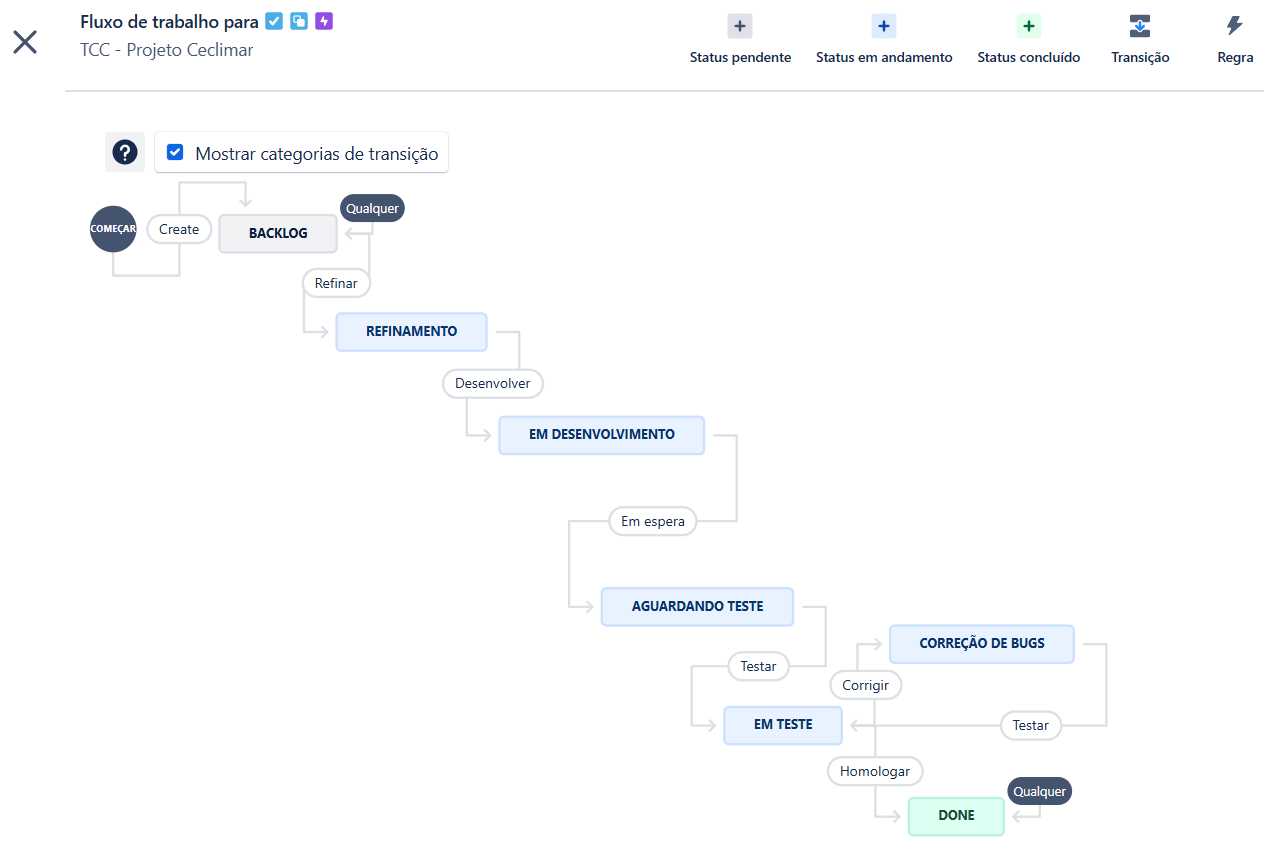
\includegraphics[width=0.8\textwidth]{imagens/fluxoJira.png}
    \caption{Fluxo de trabalho do \textit{Jira} gerado para o desenvolvimento do projeto.}
    \legend{Fonte: Autor}
    \label{fig:fluxoJira}
\end{figure} 

O \textit{Backlog} é a coluna onde todas as tarefas, \textit{user stories} e \textit{bugs} serão inicialmente 
posicionados. Nesta etapa, as tarefas serão priorizadas antes de andarem para o próximo estágio.

No Refinamento, as tarefas puxadas do \textit{Backlog} são detalhadas para um desenvolvimento 
mais assertivo. São refinados critérios de aceitação, estimativas de tempo e algum débito técnico.

As tarefas que estiverem em desenvolvimento são as que tiveram, efetivamente, o seu 
desenvolvimento iniciado. Assim que o desenvolvimento estiver finalizado, as tarefas 
serão transferidas para aguardando teste, onde ficarão até serem puxadas para testes 
mais detalhados.

No estágio de teste, os critérios de aceite e a presença de \textit{bugs} serão 
testados com o intuito de manter a qualidade do produto final. As tarefas que tiverem 
\textit{bugs} ou divergências de regras de negócio identificadas serão movidas para a coluna 
Correção de \textit{bugs} para que sejam corrigidas.

E, por último, após a homologação das tarefas nas etapas anteriores as tarefas 
são movidas para \textit{Done} que indicará sua finalização.
